\chapter{Introduction}

\eg is an open-source mesh generation software with CFD applications in mind.
\eg uses the NETGEN \cite{netgen:2008} library for tetrahedral grid generation
and an in-house development for prismatic boundary layer grids. Internally, \eg
uses the VTK \cite{vtk:2008} data structures as well as the {*}.vtu file format.
To create grids for
Currently \eg cannot generate surface grids. In order to create a volume grid it
is required to import an existing surface mesh. Gmsh \cite{gmsh:2008} is an
excellent open-source tool to create surface triangulations for \eg. Gmsh is
able to import STEP and IGES files and it can also be used for simple geometry
modelling. 

The \egv release of \eg provides native export to
OpenFOAM\textsuperscript{\textregistered}\footnote{\foam is a registered trade
mark of OpenCFD\textregistered Limited}\cite{openfoam:2008}. For future
releases, export capabilities for complete \foam cases (including boundary
conditions) and support for polyhedral cells are planned as well.

\eg is released under the GPL and we hope that it is a useful addition to the
open-source CFD community. So far the implemented algorithm proved to be quite
robust and it does not require much user interaction. Figure
\ref{fig:Introduction1}shows a boundary layer grid that has been created around
the geometry of what could be a toy plane.

\important
{
  This manual is very much a work in progress and does
  not claim to be finished, comprehensive, complete, or anything else.
  We hope that, even in this early stage, it offers a little help while
  using \eg!
}


\begin{figure}
\begin{centering}
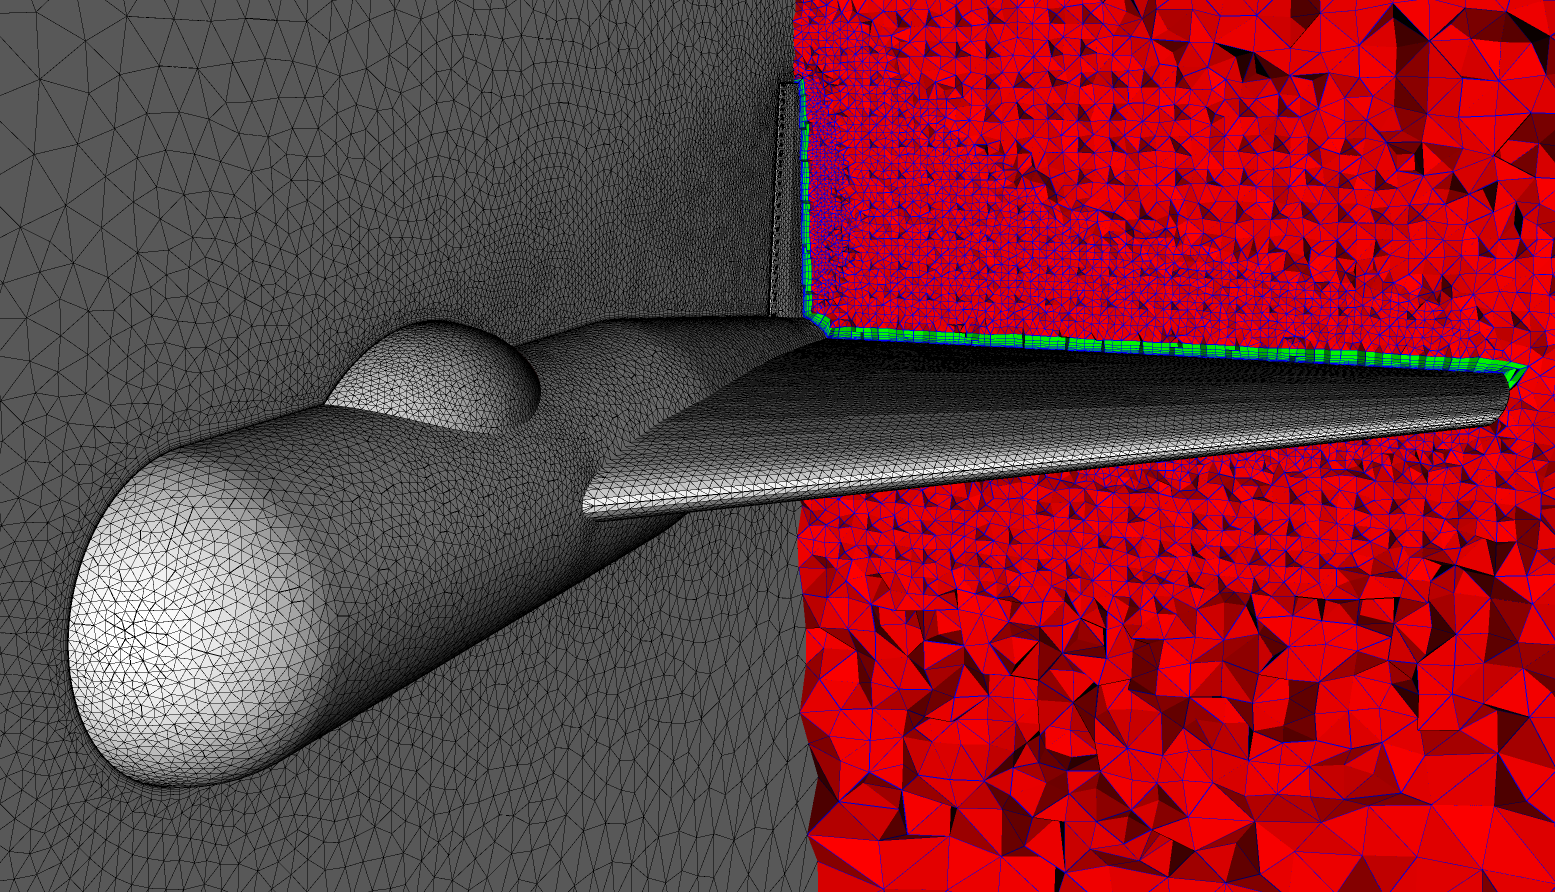
\includegraphics[width=7cm]{figures/DeltaWing_02}
\hspace{2mm}
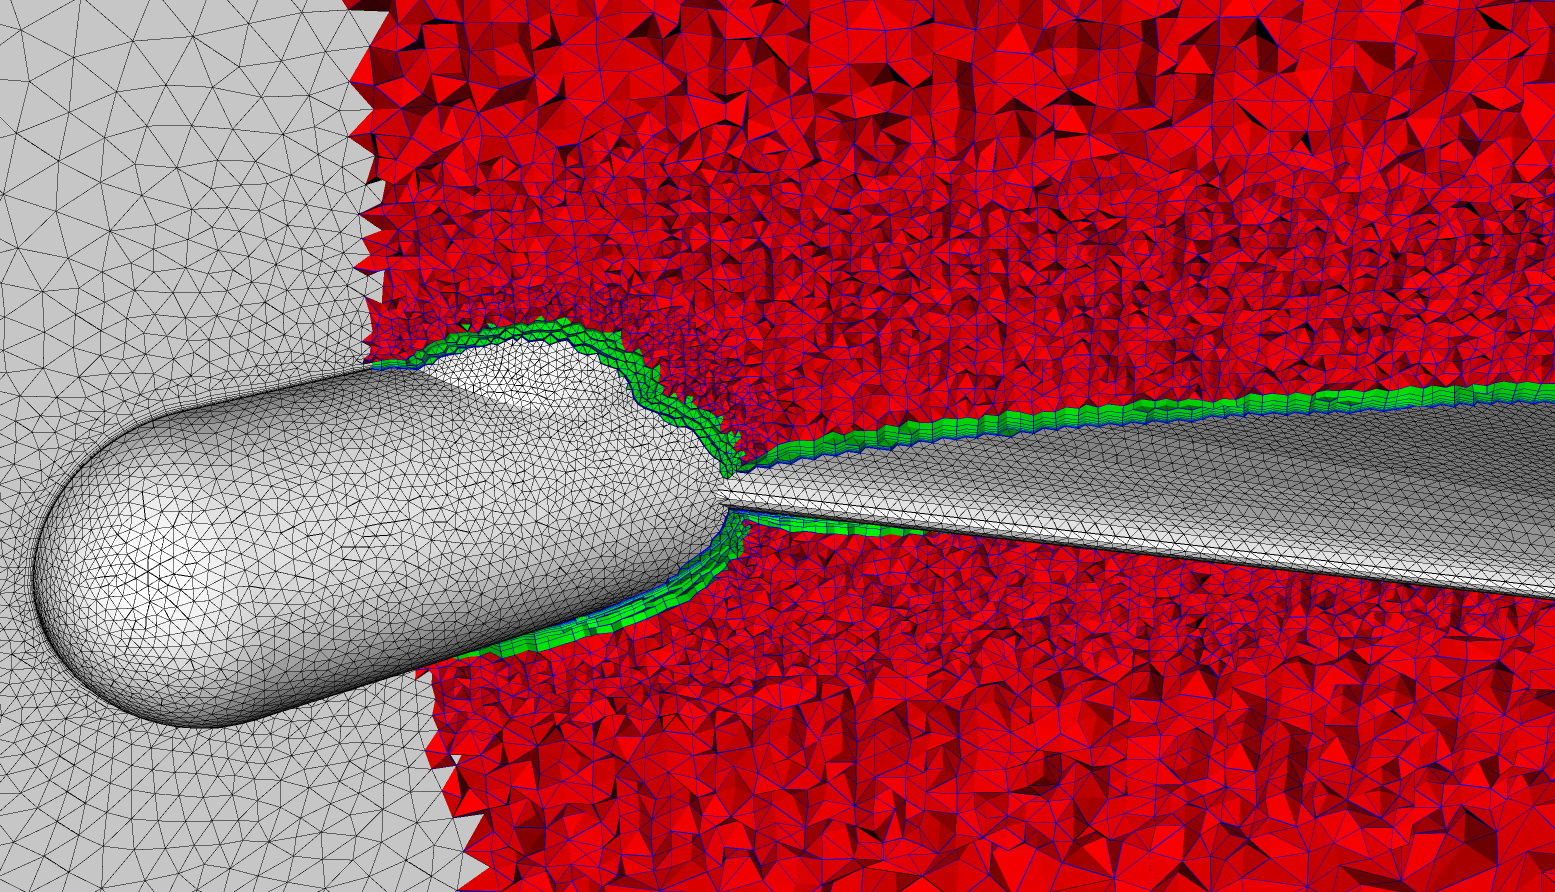
\includegraphics[width=7cm]{figures/DeltaWing_01}\\
\end{centering}
\caption{Prismatic boundary layer created by \eg}
\label{fig:Introduction1}
\end{figure}

\section{Current Release (\egv)}

\begin{itemize}
\item volume grids from existing surface triangulations (no surface meshing
support yet, but planned for future releases)
\item prismatic boundary layer support
\item GUI based on Qt4
\item direct export to OpenFOAM
\item experimental support for polyhedral grids in OpenFOAM
\end{itemize}

\section{Supported Platforms}

\begin{itemize}
\item \eg is developed on a LINUX system (OpenSUSE 10.3), using Qt-4.4.1,
VTK 5.2, and an SVN snapshot of NETGEN.
\item A Windows executable for Windows-XP (32bit) is also available.
\end{itemize}

\section{Supported File Formats}

\begin{itemize}
\item VTK unstructured grids in XML format (\eg's native format)
\item VTK poly data in XML format (import)
\item legacy VTK files (import)
\item OpenFOAM (export)
\item Gmsh (import \& export)
\item STL (import \& export)
\item NETGEN neutral format (export)
\end{itemize}


